\section{Dataset}
      \label{sec:dataset}

      \subsection{Binding Precedents}

            Until June 2021, 58 Binding Precendents have already been created. For example, take a look at BP 10's statement:

            \textit{``Viola a cláusula de reserva de plenário (CF, artigo 97) a decisão de órgão fracionário de tribunal que, embora não declare expressamente a inconstitucionalidade de lei ou ato normativo do Poder Público, afasta sua incidência, no todo ou em parte.''}
            
            The statements are short, in general, but in legal language (and in Portuguese). Although it can lead to some insights, we are not interested in studying the meaning of BP's statements.

      \subsection{Dataset description}

            The dataset used throughout this work is composed of decisions generated by STF that cite at least one Binding Precedent. Although these documents are public, they are very difficult to be accessed, mainly when it is necessary a large amount of data. This way, we use a dataset gathered in the context of Supremo em Números project \cite{falcao2013relatorio}, from FGV's Law School.

            The dataset, in the way we have it, is composed of 58 CSV files of structured data, with columns:
            \begin{itemize}
                  \item \textit{title}: document title, formed by date, document type, and an ID;
                  \item \textit{raw\_text}: document's raw text;
                  \item \textit{i\_cite}: list of cited precedents, including BPs, already extracted from the raw texts;
                  \item \textit{date}: document's publication date.
            \end{itemize}

            This is how a usual document looks like:

            \bigskip

            {\itshape``DECISÃO

            AGRAVO DE INSTRUMENTO. PROCESSUAL CIVIL. PERDA SUPERVENIENTE DO OBJETO. RECURSO ESPECIAL PROVIDO PARA ANULAR O ACÓRDÃO RECORRIDO. AGRAVO DE INSTRUMENTO PREJUDICADO.

            Relatório

            1. Agravo de instrumento contra decisão que não admitiu recurso extraordinário interposto com base no art. 102, inc. III, alínea a, da Constituição da República. (...)''}

      \subsection{Exploratory data analysis}

            Although our dataset is very simple (few, self-explanatory columns), we can analyze it more deeply to better understand it. Let's start, for example, by checking how many citations each BP has.

            \begin{figure}[H]
                  \centering
                  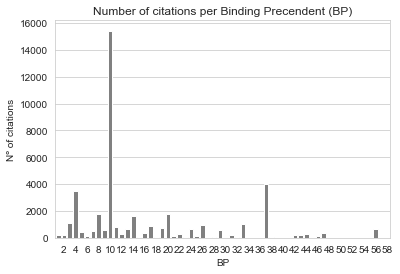
\includegraphics[width=\linewidth]{bp_citations.png}
                  \caption{Histogram of citations per Binding Precedent.}
                  \label{fig:bp_citations}
            \end{figure}

            From \autoref{fig:bp_citations}, we see that the number of citations per BP is not uniform. BP 10, for example, has the largest number of citations, followed by 37, 4, and 8. This large difference in the citation number can impact our analysis if we don't work around it.

            We already know the documents are long, but one could want to know how long these documents are. If we split each document at whitespaces and newlines and count the number of ``words'', we have a document word count distribution estimate.

            \begin{figure}[H]
                  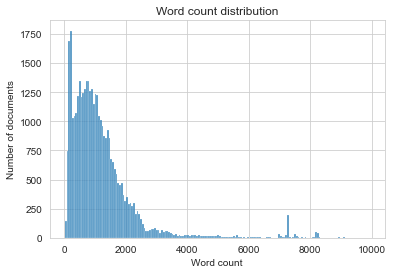
\includegraphics[width=\linewidth]{word_count.png}
                  \caption{Estimate of document word count distribution.}
                  \label{fig:word_count}
            \end{figure}

            There are some special documents (more than 10k words), but their analysis is not our focus. \autoref{fig:word_count} shows that, in general, documents are shorter than 6k words, with a mode around 1k.

            Although document titles are unique, many documents share the same raw text. This ``duplicate'' rate is around 11\%, and can also impact our subsequent analyses. This way, we need to work around these duplicated documents before fitting our models.

            Finally, one could want to see the distribution of publication date, presented in \autoref{fig:dates}. Date distribution has support between 2003 and 2018 (not clear in the plot), but it is concentrated between 2008 and 2018. It is clear that many documents have the publication year 1970, however, this information acts as a missing value. Although this is problematic, that is, many documents do not have a publication date, it will not impact our models, because we only work with raw texts.

            \begin{figure}[H]
                  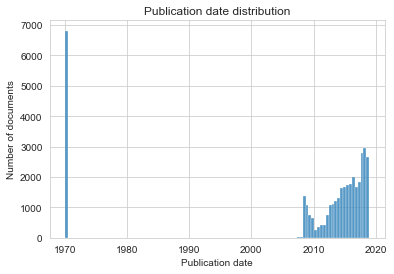
\includegraphics[width=\linewidth]{dates.png}
                  \caption{Distribution of document publication date.}
                  \label{fig:dates}
            \end{figure}
            